In this paper, Fuzzy-Logic based and arduino improved simulation project developed. In the simulation project there is independent rabbit AI's and a deer family are used to create fuzzy logic systems with dual behaviours . There is also arduino based physical control tool/device developed to make user control a flying object called eagle(Player itself)  . The AI implemented animals are acting according to the players actions . If eagle approaches to the rabbit fast and directly, rabbit tries to find an escaping route away from eagle and other possible dangers if there is one. But, rabbit changes its behaviours according to the caution range and danger range (See Fig. \ref{fig:range} ) . Also, animals can interact with each other closely too unless one side is predatory just like in a real ecology.


\begin{figure}[ht]
    \centering
    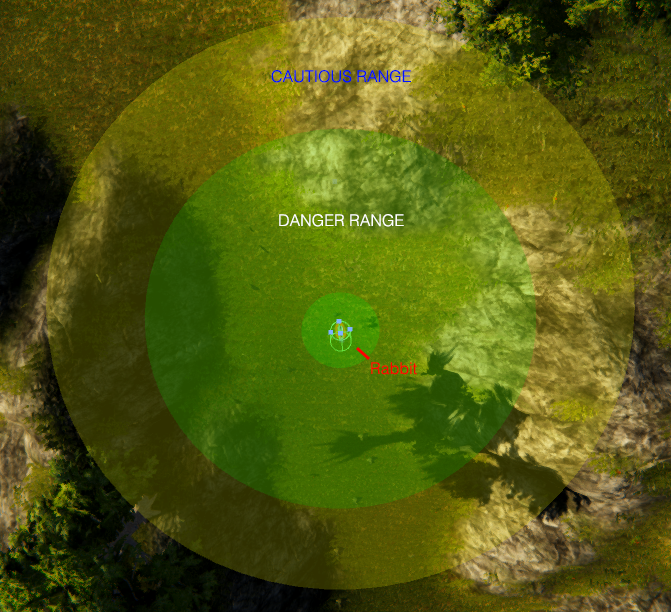
\includegraphics[scale=.45]{Images/range_rabbit_edited.png}
    \caption{Colored range demonstration on rabbit example. }
    \label{fig:range}
\end{figure}


The AI is applicable to another animals too . The only thing what user needs to do is some configuration. As we mentioned in the title of this paper there is dual behaviours what is bonded to the user's selection such as Passive , Cautious and Aggressive.

\subsection{Behaviour Types} \label{behaviour_types}


An AI's temperament controls various settings of how an AI reacts to targets or interacts with the environment and other animals/AI's. This project makes it easy by having 3 preset behaviours that AI can follow . They also have confidence level that provides you further control to make your AI's behaviour more customizable and unique. AI's use of confidence level takes shape according to behaviour type .  Below , these features will be detailly explained .

\subsubsection{Passive}
Passive AI doesn't attacks. Basically, just wanders and grazes . If they are attacked, they will react according to their confidence level .

\subsubsection{Cautious}
Cautious AI can either flee or act depending on events are happening around according to their confidence level . Any AI which have this behaving type can behave territorial if its confidence level is brave or higher.

\subsubsection{Aggressive}

This type of AI's will attack to any type of target in their target . Logically they should have great confidence .


\subsection{Confidence Levels} \label{confidence_level}
The AI does behaves according to its confidence level on its behaviour type . So , each confidence type is categorized by behaviour types .

\subsubsection{Cowardly}

\begin{table}[ht]
    \centering
    \begin{tabular}{|c|L|}
         \hline 
         Behaviour Type   & Description  \\
         \hline
         Cautious    & Flees when encounter a target in their defined range . \\
         \hline
         Passive    & Wanders around and flees when attacked . \\
         \hline
         Aggressive & Can't set to coward. Automatically start on Brave . \\
         \hline 

    \end{tabular}
    \hfill
    \caption{ Description of behaviour changes in coward confidence. }
    \label{table:cowardly}
\end{table}


\subsubsection{Brave}

\begin{table}[ht]
    \centering
    \begin{tabular}{|c|L|}
         \hline 
         Behaviour Type   & Description  \\
         \hline
         Cautious    &  When a possible target enters his radius the AI will triggered. If the possible target doesn't leave the radius within the predefined time the AI will attack to the target. And will attempt to flee when its health reaches to the limit defined. \\
         \hline
         Passive    &     Wanders around. Only attacks when attacked . And will attempt to flee when its health reaches to the limit defined. \\
         \hline
         Aggressive & Will fight with any target in its radius but attempt to flee once its health reduces to the limit defined . \\
         \hline 

    \end{tabular}
    \hfill
    \caption{Description of behaviour changes in brave confidence.}
    \label{tab:brave}
\end{table}

\newpage

\subsubsection{Overbold}

\begin{table}[ht]
    \centering
    \begin{tabular}{|c|L|}
         \hline 
         Behaviour Type   & Description  \\
         \hline
         Cautious    & When a possible target enters his radius the AI will triggered. If the possible target doesn't leave the radius within the predefined time the AI will attack to the target. This AI never flees and continues to fight until dead or the target leaves the radius fastly . \\
         \hline
         Passive    &  Wanders around and never attacks unless being attacked. This AI will never flee and continue to fight until dead or the target has leaved the radius fastly .\\
         \hline
         Aggressive & Will fight with any target in sight and will never flee. Will continue to fight until dead or the target has leaved the radius fastly  \\
         \hline 

    \end{tabular}
    \hfill
    \caption{Description of behaviour changes in overbold confidence.}
    \label{tab:overbold}
\end{table}

\subsection{Fuzzy System In The Simulation}

The project that presented in this paper has an editorial features . Hence , the inputs  can be configured . In this project health, behaviour type and confidence level are defined as the inputs into fuzzy logic system  and action states are calculated according to inputs as outputs.There are three different fuzzy techniques, known as the Mamdani \cite{:/content/journals/10.1049/piee.1974.0328}, Tagaki-Sugeno \cite{SUGENO198815} and Tsukamoto \cite{tsukamoto} fuzzy models. In this project, mamdani is used as the technique for the system also the triangular membership function used for the inputs and output .\\

Confidence Level has three membership sets : Coward , Brave and overbold. Behaviour Type also has 3 membership sets : Cautious , Passive and Aggressive. Laslty , health has 5 membership sets very low, low,medium,high and very high. Check either sections of \ref{behaviour_types} and \ref{confidence_level} or the figures of Fig.\ref{fig:health} , Fig.\ref{fig:behaviour_type} and Fig.\ref{fig:confidence_level} .\\






\begin{figure}[ht]
    \centering
    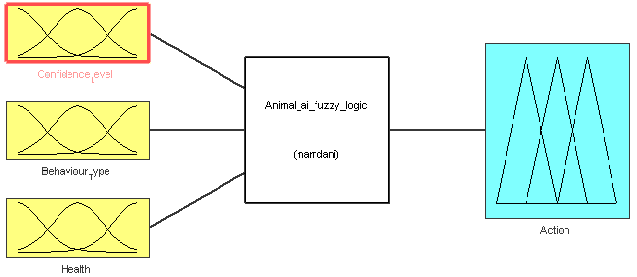
\includegraphics[scale=.53]{Images/overview.png}
    \caption{Overview of the Fuzzy Logic System}
    \label{fig:overview}
\end{figure}

Four output 4 action states define membership sets. These states are: Flee , Attempt to Flee , Wander and Fight  . Braver confidence  , higher health and more aggressive behaviour types means actions are more concentrated on fight. In adversed situation the actions are more concentrated on flee . All those outputs are calculated by the fuzzy logic system according to intensity of the states .

\begin{figure}[ht]
     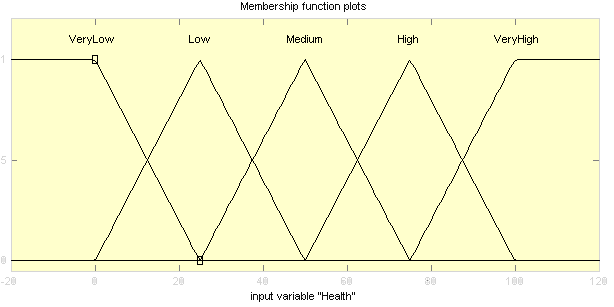
\includegraphics[width=0.5\textwidth]{Images/health.png}
    \caption{Membership Sets for Health}
    \label{fig:health}

\end{figure}

\begin{figure}[ht]
    \centering
   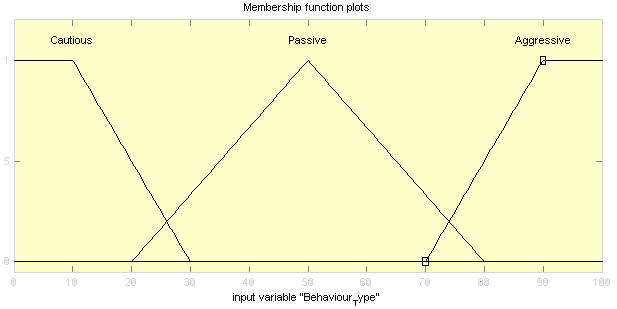
\includegraphics[width=0.5\textwidth]{Images/behaviour_type.png}
    \caption{Membership Sets for Behaviour Type}
    \label{fig:behaviour_type}
\end{figure}

\begin{figure}[ht]
    \centering
    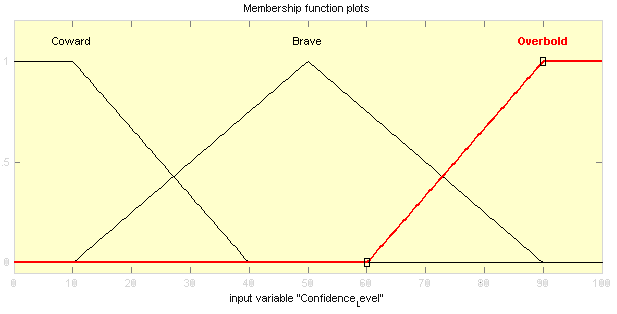
\includegraphics[width=0.5\textwidth]{Images/confidence_level.png}
    \caption{Membership Sets for Confidence Level }
    \label{fig:confidence_level}
\end{figure}

\begin{figure}[ht]
    \centering
    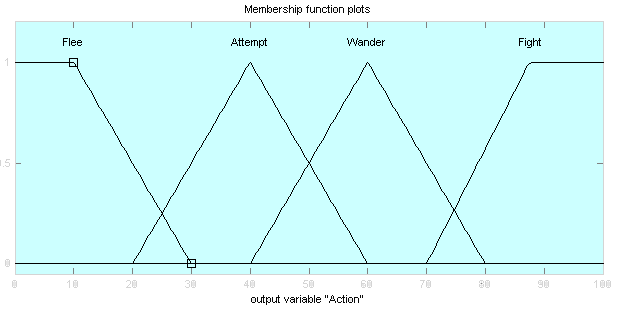
\includegraphics[scale=.55]{Images/output.png}
    \caption{Output}
    \label{fig:my_label}
\end{figure}


\clearpage

\subsection{Generating The Rules}

In order to be sure that the fuzzy system will be able to respond it's vital to create rules which cover every possibility according to sets of inputs. In case of missing there will not be any output.

The way of creating the rules is using if-then statements. For two of the input variables we have three membership sets (behaviour type and confidence level) and for the other input variable we have five membership sets which reveals the total number of the rules 3$\times$3$\times$5=45 . Since , it's not logical to have aggressive behaviours for coward animals its totally blocked to configure the system as coward and aggressive at the same time . Therefore the number of the rules decreases to 40 .



Some rules that are written for the fuzzy system are given below :\\
IF (Confidence\_Level IS OVERBOLD) AND (behaviour\_type IS CAUTIOUS) AND (Health IS VERY LOW) THEN (action IS FIGHT)\\
IF (Confidence\_Level IS COWARD) AND (behaviour\_type IS PASSIVE) AND (Health IS MEDIUM) THEN (action IS ATTEMPT TO FLEE)\\
IF (Confidence\_Level IS BRAVE) AND (behaviour\_type IS PASSIVE) AND (Health IS MEDIUM) THEN (action IS WANDER)\\
IF (Confidence\_Level IS BRAVE) AND (behaviour\_type IS AGGRESSIVE) AND (Health IS VERY HIGH ) THEN (action IS FIGHT)\\
IF (Confidence\_Level IS COWARD) AND (behaviour\_type IS CAUTIOUS) AND (Health IS LOW) THEN ( action IS FLEE)
...

The rule table which shows all rules in one combined table shown in Table \ref{T:peak} below .

\begin{table}[ht]

\scalebox{0.84}{

\begin{tabular}{|m{5em}|c|c|c|c|c|c|}
\hline
\multirow{2}{*}{Confidence}  & Behav. T.& \multicolumn{4}{c}{HEALTH}& \\
\hhline{~~-----}
                        & &Very Low&Low&Medium&High&Very High\\
\hline


\multirow{3}{*}{Coward} & Cautious & Flee &Flee &Flee &Flee &Flee \\
\hhline{~------}
                        & Passive &Flee  &Flee  &Attempt  &Wander &Wander\\
 \hhline{~------}
                        & Aggressive&- &- &- &- &-\\ %can't set to coward
\hline

\multirow{3}{*}{Brave} & Cautious &Flee  &Attempt&Wander &Fight & Fight \\
\hhline{~------}
                        & Passive &Attempt &Wander  &Wander  &Fight &Fight\\
 \hhline{~------}
                        & Aggressive&Attempt& Wander&Fight &Fight &Fight\\
\hline


\multirow{3}{*}{Overhold} & Cautious &Fight & Fight&Fight &Fight &Fight \\
\hhline{~------}
                        & Passive &Fight & Fight & Fight &Fight &Fight\\
 \hhline{~------}
                        & Aggressive& Fight &Fight &Fight &Fight &Fight\\
                        
\hline

\end{tabular}
}
\hfill

\caption{Rule Table }

\label{T:peak}

\end{table}



As clearly seen on the rule table there is no output where animal is coward and aggressive at the same time . And, as the confidence severity and health degree increases the output aims through the 'Fight' but unlike that as the both variables decreases the output aims through the 'Flee' . But , there is a third factor which affects the output and its Behaviour type which shown at the second column of the table . As the animal becomes aggressive behaviours tends to be aggressor too .

The effects made by inputs on outputs explicitly shown in the Fig. \ref{fig:surface} and Fig. \ref{fig:pseudo} .These graphics created using Fuzzy Logic Toolbox-FIS Editor-Surface Viewer in Matlab R2012a. 


\begin{figure}[ht]
    \centering
    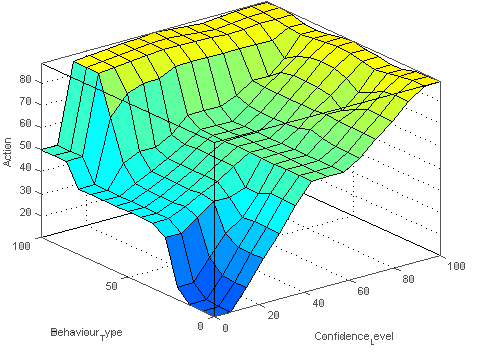
\includegraphics[width=0.52\textwidth]{Images/surface.png}
    \caption{Effects on outputs made by inputs.}
    \label{fig:surface}
\end{figure}

\begin{figure}[ht]
    \centering
    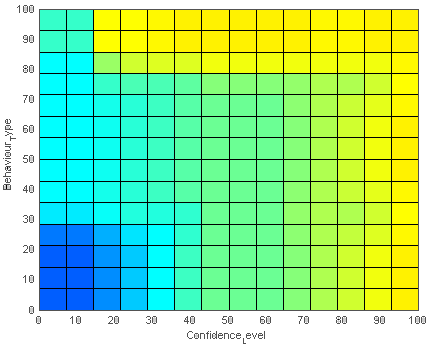
\includegraphics[width=0.5\textwidth]{Images/pseudo-color_1.png}
    \caption{Pseudo-Color type plotting.}
    \label{fig:pseudo}
\end{figure}

The Fig. \ref{fig:surface} created using plot type 'surface' and the Fig. \ref{fig:pseudo} created using plot type 'Pseudo-Color'. On the Fig \ref{fig:surface} which is 3D the output values can be seen according to behaviour type , confidence level and health . On the other hand  ,  on the Fig. \ref{fig:pseudo} Confidence Level placed at \textit{x} axis and Behaviour type placed at \textit{y} axis -also there is health on z axis but since this is pseudo type plotting only two type of values can be shown by using the (Matlab) plotter mentioned . Based on these input values the output values shown in different colors between blue and yellow.

By using the Rule Editor in FIS Editor , all the ruled used in the fuzzy logic system and their outputs as reaction can be watched easily.  For example , two different calculations can be examined in Fig.\ref{fig:example}


\subsection{Action System}

After getting all needed information according to health, behaviour type and confidence level of animal the fuzzy system triggers all the functions to reach animations and models . And plays the animations depending decided -by AI itself- action . If animal loses too much health its action starts to move through flee from other action states depending on its confidence level too. The animal AI never loses or changes its confidence level according to any incident .

See Fig. \ref{fig:example} to see fuzzy system with membership degrees of inputs and output . The animals for different action states  as explained :\\


\begin{itemize}
    \item if the action state is \textit{fight} ,then AI starts a countdown to let the other animal(s) leave its range before attacking , the limits of counter can be defined in editor  . If animal in range doesn't leave the range within the countdown then the AI checks its attacking animations and gets closer range of its enemy to be able to fight and use  animations properly to give damage , if AI loses so much health and can't make its enemy run-away then action morphs from \textit{fight} to less aggressive actions step by step like :\\
    
    \textit{fight} $>$   \textit{wander}  $>$ \textit{attempt to flee} $>$  \textit{flee} .\\
    
    
    Unlike all those informations when animals confidence is \textit{overbold} the AI never flees or changes it action states from fight to anything else . Basically ,  fights till die. \\
    
    \item if the action state is \textit{wander} , it starts to wander around unless it sees another wild animal in sight
    . If there is a wildly-acting animal in sight it starts to move faster around and tries to find alternative ways around to become distant from wild animal(s).\\
    
    \item if the action state is \textit{attempt to flee}, it calculates a quick route to flee from fight to become distant from its enemies . Its the step where animal just tries to beware from a on-going fight to stop taking damages . Most likely, after this step animal will flee .\\
    
    \item if the action state is \textit{flee} , it starts to calculate quick routes to save its life and beware from the possible fights . This action is the worst situation that an animal can experience in this simulation particularly when the confidence is brave . Because, when confidence level is coward the AI flees from everything . But, when its brave and AI choose to flee it means that animal had damage and just trying to save its life . In this case , if animal couldn't succeed to flee then it becomes a open target for the wild animals in close range especially for the ones AI was trying to flee from .
    
    
\end{itemize}

\hfill



\newpage

\begin{figure}[ht]
  \subfigure[ Confidence Level=87.1 Behaviour Type=84.2 Health=89.4 and Action=87 ]{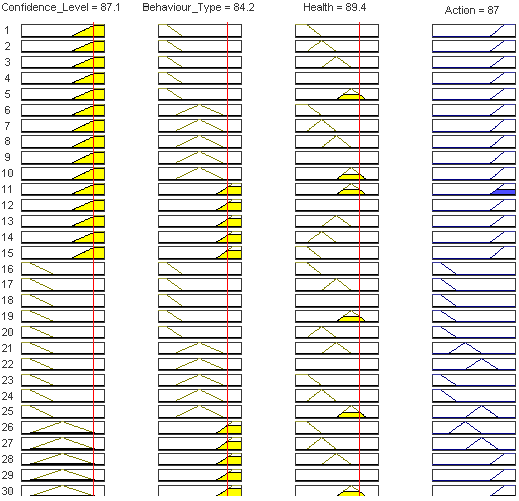
\includegraphics[width=0.5\textwidth]{Images/example_1.png}}\\
  \subfigure[Confidence Level=23.2 Behaviour Type=38.8 Health=6.65 Action=32.3 ]{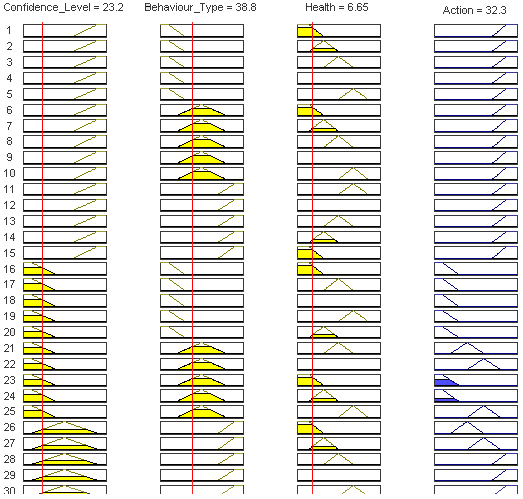
\includegraphics[width=0.5\textwidth]{Images/example_2.png}}
  \caption{Two Different Examples}
  \label{fig:example}
\end{figure}


As its very clear to understand , only confidence level, health and behaviour type affects the action states. The membership degrees of all those actions can change according to the changes in those inputs . But , its impossible to change an action state totally from one to another . Animals can't gain health with any condition .
\newpage

